\documentclass[tikz,border=10pt]{standalone}
\usepackage{amsmath}
\begin{document}
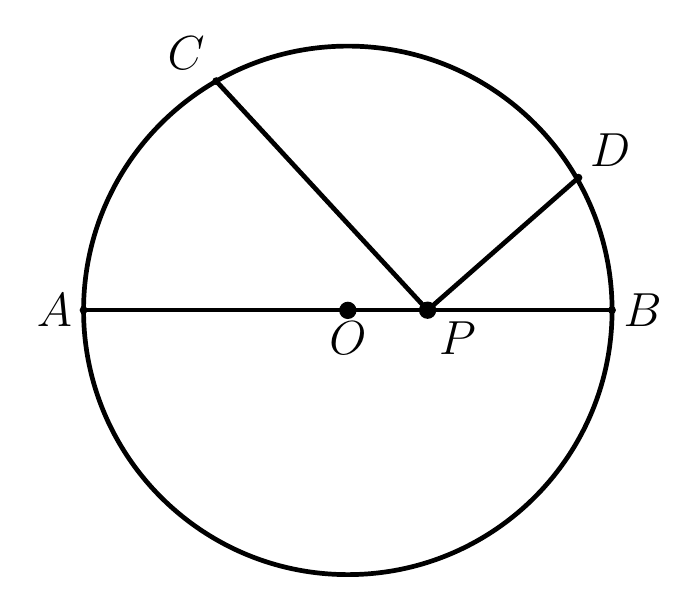
\begin{tikzpicture}[line width=1.7pt, line join=round]
\coordinate (A) at (-3.382,-0.149);
\coordinate (B) at (3.329,-0.149);
\coordinate (C) at (-1.697,2.759);
\coordinate (O) at (-0.026,-0.152);
\coordinate (P) at (0.987,-0.150);









\coordinate (D) at (2.903,1.533);


\draw (O) circle (3.356);


\draw (A) -- (B);
\draw (C) -- (P);
\draw (P) -- (D);


\foreach \X in {A,B,C,D}
  \fill (\X) circle (0.050);
\fill (O) circle (0.110);
\fill (P) circle (0.110);


\node[left] at (A) {\fontsize{17}{20.4}\selectfont $A$};
\node[right] at (B) {\fontsize{17}{20.4}\selectfont $B$};
\node[below] at (O) {\fontsize{17}{20.4}\selectfont $O$};
\node[below right] at (P) {\fontsize{17}{20.4}\selectfont $P$};
\node[above left] at (C) {\fontsize{17}{20.4}\selectfont $C$};
\node[above right] at (D) {\fontsize{17}{20.4}\selectfont $D$};
\end{tikzpicture}
\end{document}